% !TeX spellcheck = sk_SK
\mychapter{2}{Opis riešenia - Workflow systém}

%\centerline{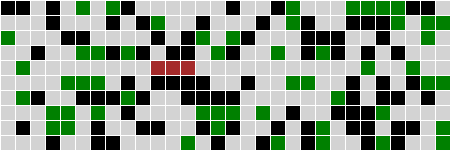
\includegraphics[width=0.4\textwidth]{images/cervik}}


%klucove slova ... špecifikovať, analyzovať , poukázať, predstaviť, vytvoriť, rozobereať, načrtnúť
\section{Špecifikácia požiadaviek}
%V nasledujúcej sekcii opíšeme základný model fungovania aplikácie, analyzujeme  požiadavky a naznačíme spôsob jej realizácie. Pre lepšie pochopenie aplikácie si pomôžeme jednoduchým príkladom procesu, na ktorom vyniknú hlavné výhody nášho systému. V rámci nášho systému sa špeciálne zameriame na model riadenia systému pomocou rolí.  

\subsection{Základný opis aplikácie}
Zistili sme, že workflow management systém je silný nástroj, ktorý umožní používateľovi oddeliť a jasne znázorniť procesnú časť od aplikácie. Tento systém ponúka mnohé výhody. Jednou z možností ako WfMS implementovať je použitím Petriho sietí. Petriho siete sú jasne formálne definované a matematicky overené.  Rozhodli sme sa preto implementovať Petriho siete ako nástroj pre modelovanie procesov.\\

Celý systém bude fungovať na portáli, cez ktorý bude možné sa registrovať a následne prihlásiť. Aplikáciu môžeme pomyselne rozdeliť na modelovaciu a používateľskú časť (obrázok \ref{fig:model_apk}). V modelovacej časti je možné navrhovať a modelovať procesy prostredníctvom Petriho sietí . Ku ním sa v \emph{editore manažmentu rolí a organizačnej štruktúry} pripoja role a v \emph{editore formulárov a dátového modelu} sa namapujú formuláre. Takto vytvorená workflow sieť spolu s rolami a formulármi je tak pripravené na používanie. 

Pre používanie potom stačí workflow sieť nasadiť (deploy) do konkrétnej firmy. Vo firme bude potrebné priradiť konkrétnych používateľov ku rolám, ktoré táto workflow sieť používa. Následne tak môžeme považovať Workflow systém za funkčný a budeme môcť vytvárať nové prípady. Prechody sa budú dať spúšťať v každom prípade  automaticky podľa namodelovanej logiky.

	\begin{figure}[h]
		\centering
		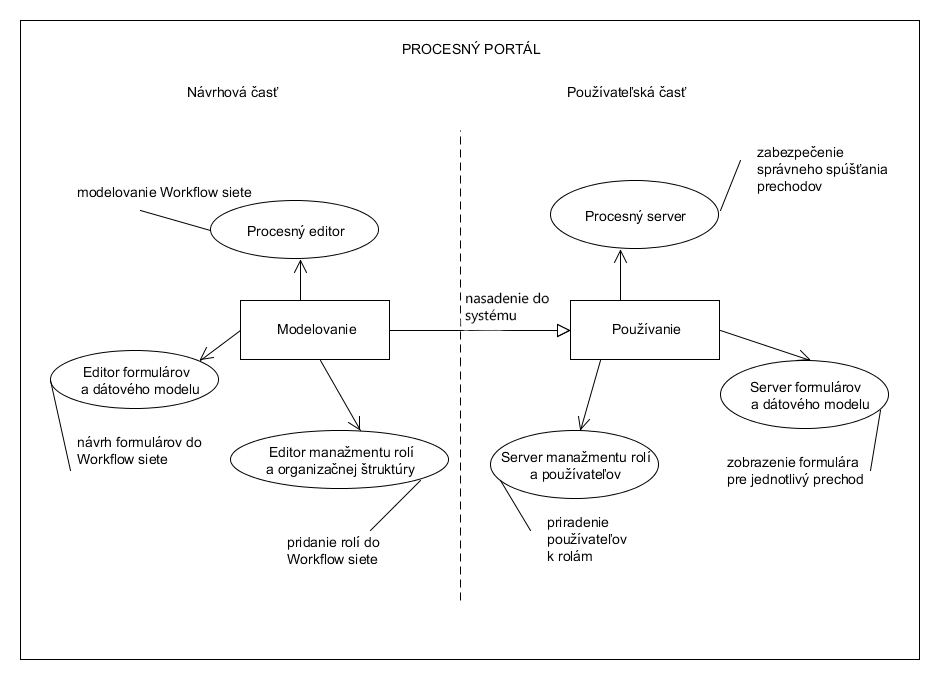
\includegraphics[width=0.9\linewidth]{images/model_apk}
		\caption{Model wokflow systému}
		\label{fig:model_apk} 
	\end{figure}



%Pri aplikácii Petriho siete na WfMS, prechody predstavujú úlohy, ktoré za sebou nasledujú v určitom poradí. Tieto úlohy môžeme rôzne definovať.  Príklad takejto úlohy je napríklad vypísanie daňového priznania, schválenie žiadosti alebo iné. V našej aplikácii bude ku každému prechodu v sieti možné priradiť formulár, ktorý pokryje väčšinu bežných požiadaviek. Pre vypísanie daňového priznania sa teda bude dať jednoducho vypísať formulár, ktorý bude obsahovať potrebné políčka ako krátka odpoveď, dlhá odpoveď, zaškrtávacie políčka prípadne výber z viacerých možností. Každú úlohu musí niekto spustiť a vykonať. Je treba teda definovať prístup riadenia v aplikácii. Pre tieto účely sme zvolili systém riadenia za pomoci rolí, ktorý sa ukázal ako flexibilné riešenie našich požiadaviek. Ku každému prechodu v procese bude okrem formuláru pridelená rola ktorá môže daný prechod spustiť. 

%Aby však daná aplikácia mohla fungovať ako plnohodnotné WfMS potrebujeme aplikačné rozhranie, ktoré bude nad vytvoreným procesom zabezpečovať jeho správne fungovanie. Naša aplikácia bude poskytovať webové rozhranie, ktoré umožní používateľom používať náš systém bez nutnosti sťahovať dodatočný softvér. Takisto sa tým vyhneme problémom spojených s kompatibilitou odlišných operačných systémov.  Na strane servera budeme využívať kombináciu jazyka PHP s databázovým systémom MySQL. Na strane klienta využijeme framework  Jquery, ktorý je rýchly a nenáročný na pamäť.\\

%Kľúčovou výhodou WfMS je možnosť oddeliť proces od aplikačnej časti. Veľa firiem používa rovnaké alebo veľmi podobné procesy. Predstavme si dve rôzne pekárne. V zjednodušenom pohľade môžeme povedať, že pre obidve pekárne platí rovnaký proces výroby chleba. Jediné v čom sa tieto pekárne odlišujú je zamestnanecká štruktúra. Náš systém by umožnil obidvom pekárňam použiť rovnaký proces. Ak je možné prepoužiť rovnaké procesy pre viacero firiem, vzniká tu možnosť procesy predávať. V našej aplikácii je preto dôležitou súčasťou portál, ktorý okrem poskytnutia tvorby procesov a jeho následného používania, poskytne možnosť vyhľadávať a prepoužívať procesy, ktoré už boli vytvorené.  


\subsection{Funkcia rolí v aplikácii}
V biznis procesoch väčšinu úloh vykonávajú fyzické osoby. V každej firme je niekoľko zamestnancov, ktorí majú rôzne právomoci. Zároveň však môžeme vidieť ich neustálu fluktuáciu. Zamestnanci do firmy prichádzajú a aj odchádzajú. Takisto sa stáva, že zamestnanec zmení pozíciu vo firme a dostane tak nové právomoci. Pre efektívny management riadenia takéhoto systému nám nestačí využitie klasických modelov, prípadne systém na správu takéhoto systému by bol vysoko nákladný. Z týchto dôvodov väčšina workflow management systémov využíva model  prístupu na základe rolí RBAC. Pre potreby našej aplikácie preto využijeme základy tohoto modelu ( konkrétne implementujeme základný model z frameworku RBAC0 \cite{sandhu96}). V každej Workflow sieti priradíme rolu na sieť, aby sme vedeli určiť, kto môže spustiť nový prípad. Zároveň v Petriho sieti definujeme ku každému prechodu jednu rolu, ktorá môže daný prechod spustiť. Samotné právomoci role nad prechodom sú určené v dátovej časti. Vo formulári ku prechodu sa dajú políčka nastaviť ako povinné, upraviteľné a viditeľné. To nám zabezpečí ekvivalent k právomociam read, write. 

\begin{figure}[h]
	\centerline{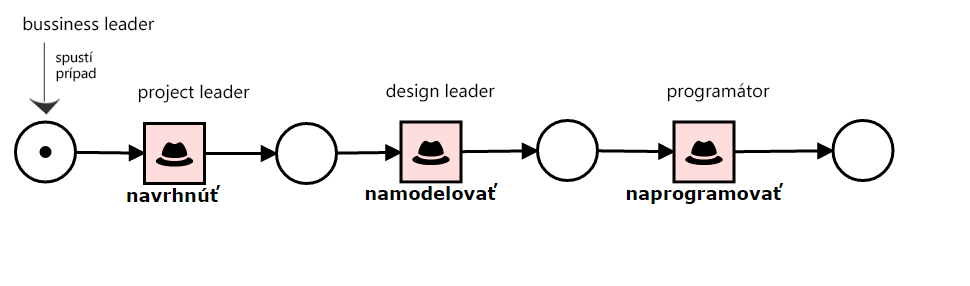
\includegraphics[width=0.9\textwidth]{images/vyvoj_role}}
	\caption{Príklad priradenia rolí k prechodom (vytvorenie novej aplikácie zjednodušene)}
	\label{obr:role_na prechody}
\end{figure}



\subsection{Referencie}
Role v procese zabezpečia prenos prístupových práv z úloh na používateľa. V rámci jednej role si môžeme predstaviť skupinu používateľov, ktorí majú určité spoločné prístupové práva vo firme. V niektorých procesoch však treba zabezpečiť, aby dve od seba závislé úlohy, mohol spustiť len ten samý používateľ. Samotné role túto funkcionalitu nedokážu zabezpečiť . V našej aplikácii je nutné ju explicitne zadefinovať. Do našej aplikácie sme použili systém referencii na prechody v Petriho sieti. Konkrétne sme implementovali dva typy referencii : \emph{referencia na prechod} a \emph{referencia na prvého používateľa z role} .\\ 

Najskôr opíšeme referenciu na prechod. Referencia na prechod zabezpečí, aby ten samý používateľ ktorý spustí prechod, na ktorý odkazuje referencia, bol jediný oprávnený na spustenie prechodu s touto referenciou. Jednoduchým príkladom je ak rozložíme jeden zložitý prechod , ktorý musí vykonať ten samý používateľ na dve menšie. Predstavme si napríklad podpísanie tlačiva (obrázok \ref{fig:referencia_na_prechod}). Ku tlačivu treba podpísať aj jeho kópiu. Náš prvý prechod predstavuje podpísanie tlačiva a druhý prechod je priradený k podpísaniu kópie tlačiva. Podpísanie kópie obsahuje v sebe referenciu na prvý prechod s podpísaním originálneho tlačiva. V praxi to znamená, že obidve tlačivá musí podpísať tá istá osoba. \\

	\begin{figure}[h]
		\centering
		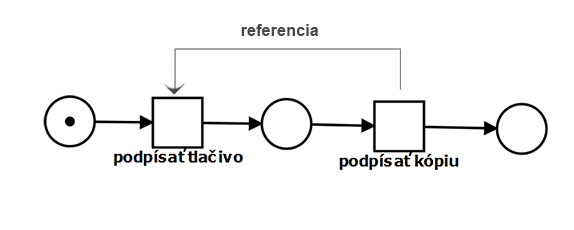
\includegraphics[width=0.7\linewidth]{images/referencia}
		\caption{Referencia na prechod}
		\label{fig:referencia_na_prechod}
	\end{figure}


V procese však môžu existovať úlohy, ktoré sa v určitom prípade nikdy nevykonajú. Príkladom v Petriho sieti je podmienené vykonanie prechodov na základe OR-splitu. V prípade, že by sme namodelovali proces s referenciu na takýto prechod, pri vykonávaní procesu by sme sa dostali do stavu, kedy by nikto daný prechod nemohol spustiť a tým pádom by nebolo možné proces ukončiť. Takýto stav by bol nežiadúci a spôsobil by mnoho problémov. Druhým problémom je, že v procese vopred nevieme určiť poradie vykonávania jednotlivých úloh. Chceme aby prechod1 aj prechod2 spustil rovnaký človek z role. Nevieme však v akom poradí budú prechody za sebou nasledovať. Z týchto dôvodov sme sa rozhodli pridať "referenciu na prvého používateľa z role". Táto referencia rieši obidva problémy zároveň. Prechod, ktorý bude označený touto referenciou , bude môcť spustiť jedine používateľ, ktorý v procese prvýkrát spustil prechod pod takou rolou, akú má prechod s referenciou. V prípade, že taká neexistuje, znamená to, že dosiaľ nebol spustený žiaden prechod, ktorý by obsahoval danú rolu. V tomto prípade bude môcť prechod spustiť ktorýkoľvek používateľ, ktorý je priradený k danej role.

\begin{figure}[h]
	\centering
	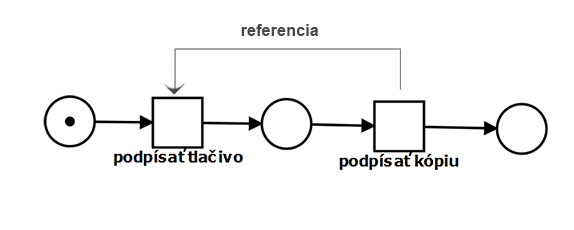
\includegraphics[width=0.7\linewidth]{images/referencia}
	\caption{Referencia na prechod}
	\label{fig:referencia na prvého z role}
\end{figure}

%teraz mi napadlo, že by bolo dobré to spraviť tak, že by bola napr. referencia1 - priradená prechodom 2,3,4 a ktokoľvek by prvý spustil hociktorý z týchto prechodov by následne určil danú referenciu. Je to taká modifikácia nášho prvý z role. Ale umožňovalo by to mať viacero referencii tej samer role v jednom procese a zjednodušilo by to systém , pretože by to fungovalo rovnako dobre aj na náš prvý prípad "referencia na prechod" 



\section{Návrh}
V nasledujúcej sekcii bližšie popíšeme jednotlivé časti systému, tak ako sme si ich rozdelili.

\subsection{Procesný portál - Martin Kováčik}
Procesný portál slúži na zjednotenie všetkých častí dohromady. Základnou myšlienkou portálu je poskytnúť možnosť vytvárať, využívať a manažovať Workflow systémy. Taktiež slúži ako e-shop. Ponúka možnosť vytvorené Workflow siete kopírovať do iných firiem. Všetky firmy a workflow siete sú verejne viditeľné. Vytvára priestor, kde sa dajú procesy vzájomne vymieňať. Vďaka tomu môžu používatelia využívať vo svojich firmách Workflow systém bez nutnej znalosti samotného modelovania Workflow siete. Portál umožňuje registráciu a prihlásenie používateľov. Prihlásený používateľ  môže manažovať svoj profil : prezerať svoje objednávky, meniť heslo. V prípade straty hesla zabezpečí jeho opätovné zaslanie. Každý používateľ môže vytvoriť a spravovať vlastnú firmu. Vo firme je zahrnutá správa používateľov. Ich pridávanie a vyhadzovanie z firmy ako aj priradenie práv na správu firmy. Nového používateľa je možné pridať do firmy cez zaslanie pozvánky. Zaregistrovaní používatelia majú vstup do firmy voľný, prípadne zabezpečený cez heslo.  V portáli je zabezpečený prístup do modelovania workflow sietí spolu s editorom manažmentu rolí a editorom formulárov, ako aj k správe rolí a ich mapovaniu na používateľov. 

\begin{figure}[h]
	\centering
%	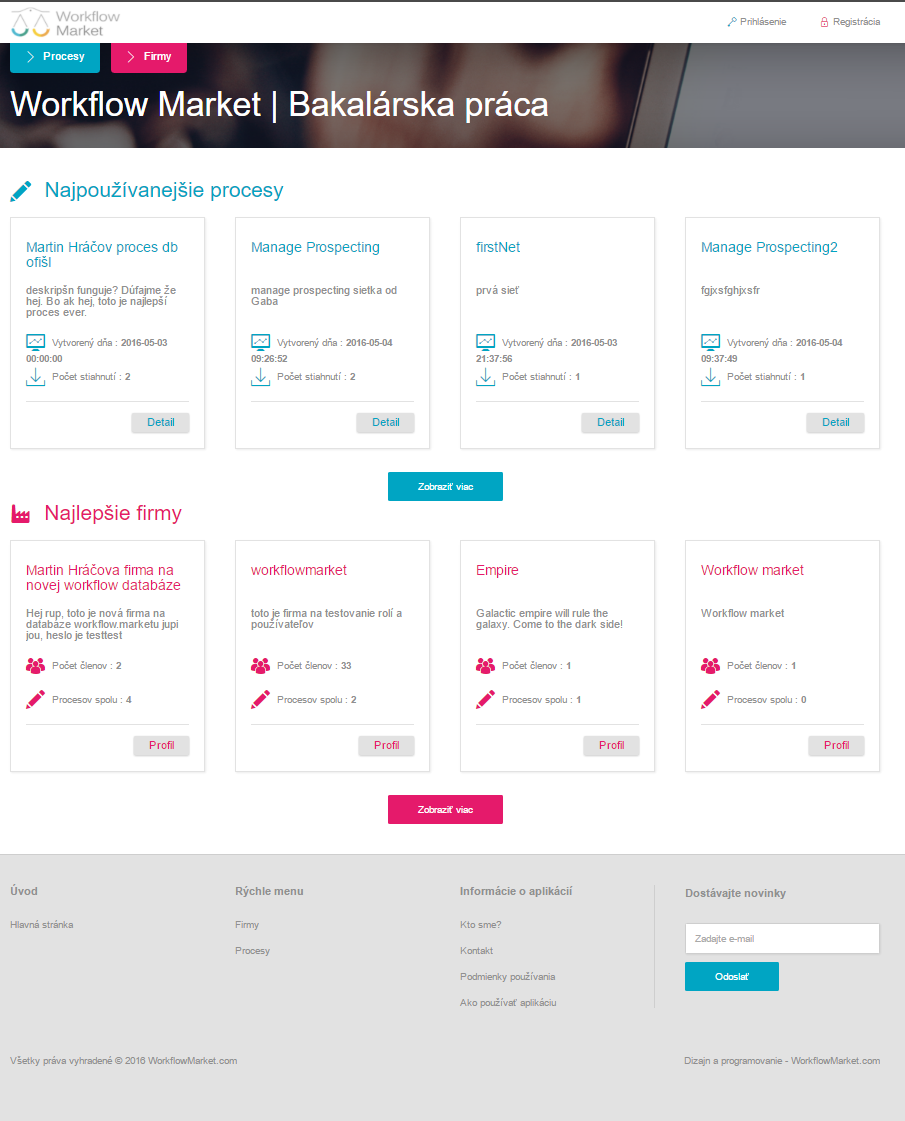
\includegraphics[width=0.7\linewidth]{images/martin}
	\caption{Procesný portál}
	\label{fig:procesný portál}
\end{figure}



\subsection{Procesný editor - Tomáš Prieboj}
Procesný editor ponúka možnosť modelovať Petriho sieť a navrhnúť tak workflow sieť pre vytvorenie firemných procesov. Nájdeme tak v ňom nástroje na kreslenie rôznych objektov ako miest, prechodov a hrán. Každý takýto objekt je možné presunúť a vymazať. Pri presúvaní je automaticky zabezpečené presúvanie hrán napojených na objekt. Vymazanie objektu analogicky zaručí odstránenie hrán, ktoré by inak nemali začiatočný alebo koncový bod. Každé miesto a prechod je možné označiť menovkou. Udeľovanie značkovania (tokenov) pre miesta je zabezpečené dvoma spôsobmi. Prvý spôsob pridáva tokeny ľavým tlačidlom myši a  pravým tokeny uberá. Druhý spôsob umožní k miestu ručne napísať počet tokenov. Dôležitou funkcionalitou je simulácia Petriho siete. Dovoľuje používateľovi simulovať proces v Petriho sieti, pričom v každom stave zobrazuje aktívne prechody. Aplikácia umožňuje ukladanie siete buď vo formáte SVG ako obrázok, alebo vo formáte XML, z ktorého je možné neskôr celú sieť importovať na účely modelovania. Pre potreby Workflow systému, editor ukladá popis workflow siete a cez komunikáciu prostredníctvom JSON-u s procesným serverom umožňuje uložiť sieť do databázy. Po uložení do databázy príjme id, ktoré bolo sieti priradené. Následne tak môže používateľa presmerovať na editor formulárov a dátového modelu.

\begin{figure}[h]
	\centering
%	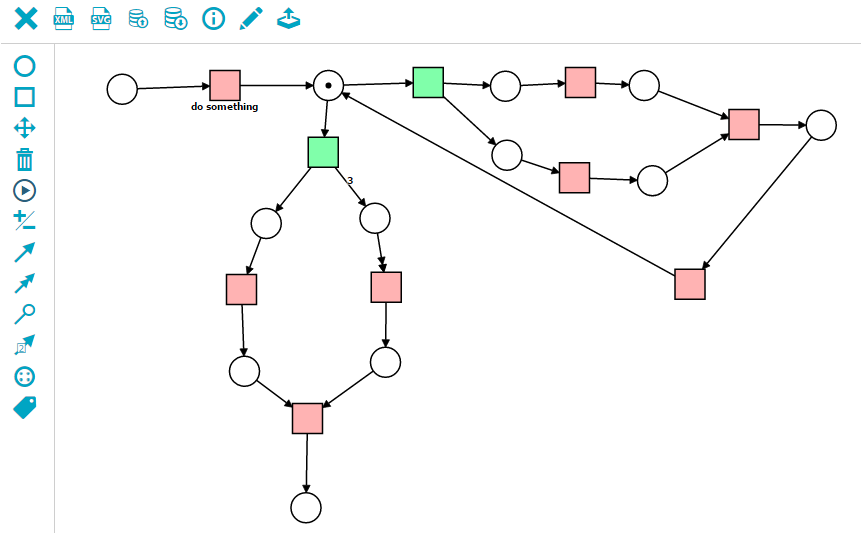
\includegraphics[width=0.7\linewidth]{images/tomas}
	\caption{Procesný editor}
	\label{fig:Procesný editor}
\end{figure}


\subsection{Editor formulárov a dátového modelu - Ján Polaček}
\label{editor formulárov}
Po tom, ako sa workflow sieť nakreslí v procesnom editore je potrebné k prechodom priradiť formuláre, ktoré sa budú neskôr zobrazovať pri spracovaní úloh v prípadoch. Editor formulárov a dátového modelu umožňuje navrhnúť dátový model pre formuláre. Modelovanie formulárov je realizované cez vytváranie, editovanie, prípadne mazanie vstupných polí. Tie môžu byť pridané v podobe \emph{krátkej odpovede}, \emph{dlhej odpovede} , \emph{výberu z viacerých} (select boxu ) 	alebo \emph{zaškrtávacích možností } (checkboxy) . Ku každému sa dá pridať otázka a popis. Pre jednotlivý vstup definujeme , či je povinný, viditeľný a upraviteľný. Pre potreby prepoužívania formulárov a ich ukladania do databázy sa vytvorí dataset, ktorý reprezentuje premenné, do ktorých sa ukladajú hodnoty z vstupných polí. Editor dokáže načítať a uložiť Petriho sieť cez formát SVG. Jednotlivé formuláre a dátové typy je možné uložiť vo formáte XML a následne spätne nahrať na načítanú sieť (napr. prostredníctvom SVG). Editor spolupracuje so \emph{serverom formulárov a dátového modelu}. Prostredníctvom JSON dát sú formuláre priebežne ukladané na server.


\begin{figure}[h]
	\centering
%	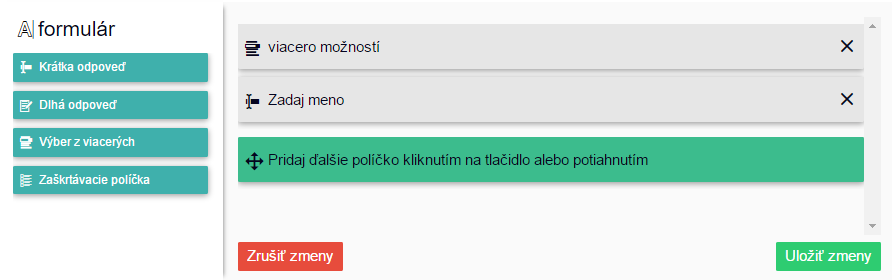
\includegraphics[width=0.7\linewidth]{images/jan}
	\caption{editor formulárov a dátového modelu}
	\label{fig:editor formulárov a dátového modelu}
\end{figure}


\subsection{Editor manažmentu rolí a organizačnej štruktúry- Kristián Stroka}
\label{Editor manažmentu rolí a organizačnej štruktúry}
Podobne ako pri editore formulárov, \emph{Editor manažmentu rolí a organizačnej štruktúry} slúži na bližšie definovanie prechodov, konkrétne sa zameriava na otázku kto môže spustiť prípad a prechody v ňom. Editor umožňuje vytvárať roly a následne každému prechodu vymedziť prostredníctvom  rol a referencii práva na spustenie prechodu. Každému prechodu je možné priradiť rolu, prípadne jednu z dvoch referencii : \emph{referenciu na prechod} a \emph{referenciu na prvého používateľa z role}. Toto priradenie je možné následne zrušiť. Editor načítava Petriho sieť prostredníctvom SVG formátu načítaním zo súboru, prípadne z databázy. Mapovanie rolí a referencii je možné uložiť v XML formáte. Pre potreby Workflow systému je ukladanie mapovania do databázy zabezpečené prostredníctvom JSON komunikácie  zo \emph{serveru manažmentu rolí a používateľov}. Rovnakým spôsobom je možné z databázy načítať roly vo firme v akej používateľ práve modeluje.

\begin{figure}[h]
	\centering
%	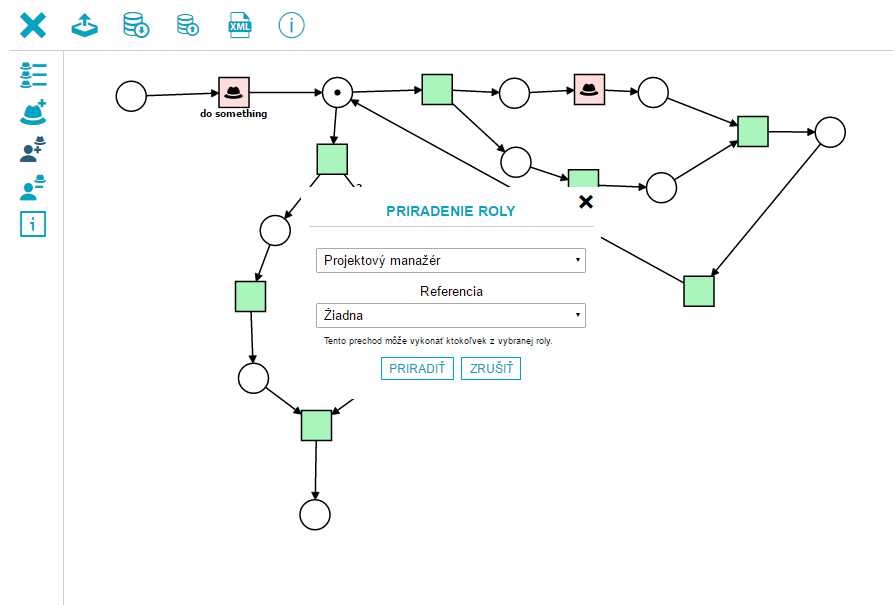
\includegraphics[width=0.7\linewidth]{images/kristian}
	\caption{Editor manažmentu rolí a organizačnej štruktúry}
	\label{fig:Editor manažmentu rolí a organizačnej štruktúry}
\end{figure}


\subsection{Procesný server - Anna Demeterová}
Procesný server zabezpečuje správne fungovanie Workflow systému po jeho namodelovaní vo firme. Pre konkrétneho používateľa vo firme zabezpečí, aby mohol vytvárať nové prípady a preberať úlohy z vytvorených prípadov podľa stavu, v akom sa prípad nachádza a používateľských oprávnení zadefinovaných na základe rolí. Stará sa tak o to, aby každý prípad nasledoval logiku definovanú namodelovanou Workflow sieťou. Kontroluje a zabraňuje možným  kolíziám referencii a iným deadlockom.  
%cancel čo? 
Ukladá históriu vykonaných prípadov a úloh. Umožňuje vizualizáciu stavu, v akom sa prípad nachádza. Okrem toho spracováva workflow siete vytvorené v \emph{procesnom editore} a ukladá vytvorenú sieť do databázy. Po prebratí úlohy používateľovi zobrazí možnosť túto úlohu vykonať. To ho presmeruje na \emph{server formulárov a dátového modelu} kde sa používateľovi zobrazí formulár patriaci danej úlohe. Ak je formulár vyplnení, odošle sa naspať potvrdenie. Procesný server tak dokončí úlohu a zabezpečí posunutie prípadu do nového stavu. Procesný portál nanovo vypočíta aktívne prechody na spustenie.

\begin{figure}[h]
	\centering
	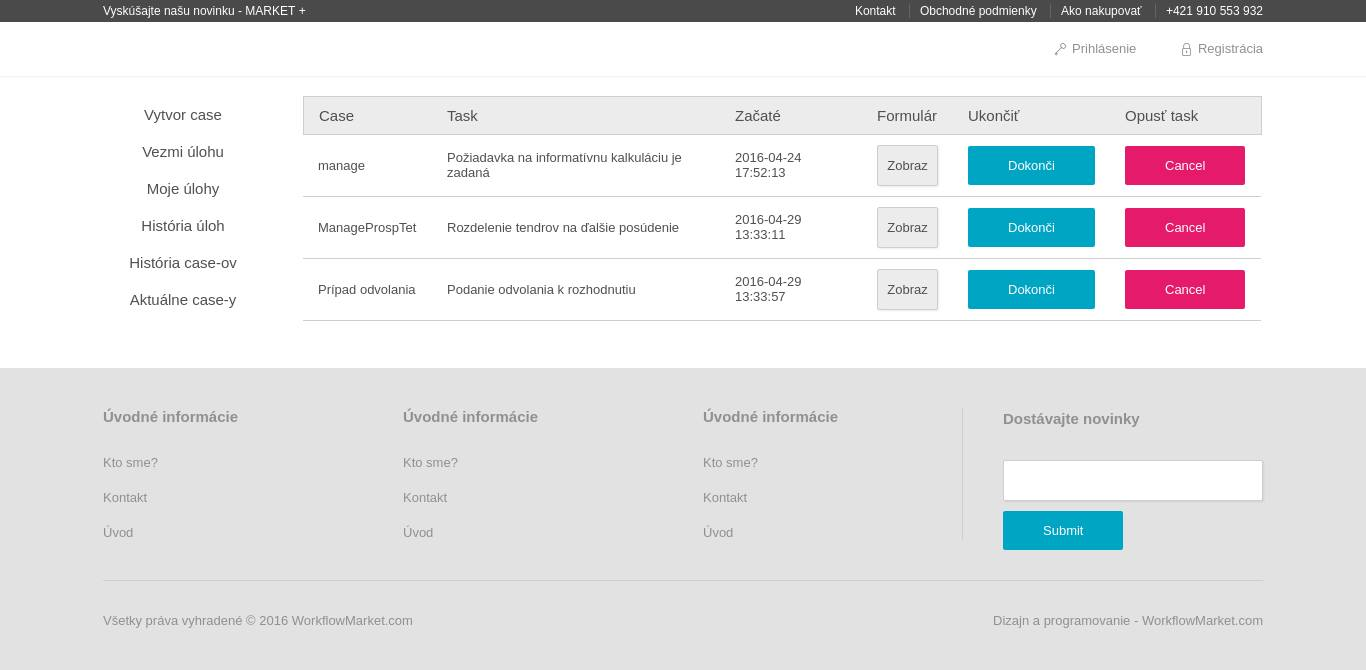
\includegraphics[width=1\linewidth]{images/anicka}
	\caption{Procesný server}
	\label{fig:Procesný server}
\end{figure}



\subsection{Server formulárov a dátového modelu- Jakub Kováčik}
Serverová strana formulárov a dátového modelu rieši zobrazovanie formulárov pre spustené úlohy v konkrétnom prípade. Formulár môže obsahovať krátku odpoveď, dlhú odpoveď, zaškrtávacie pole a výber z viacerých možností. Po odoslaní formuláru prebieha validácia, či sú vstupné polia správne vyplnené. Taktiež umožňuje priebežne uložiť vyplnené polia, bez toho aby sa formulár odoslal. To umožní používateľovi odložiť vypĺňanie na neskôr. Táto časť je pevne previazaná s editorom formulárov (\ref{editor formulárov}) . Zatiaľ čo editor rieši modelovanie dátového modelu a návrh formuláru, serverová časť sa stará o ukladanie dát a následné zrekonštruovanie formuláru pre jeho samotné vypĺňanie. Komunikácia medzi editorom a serverom prebieha prostredníctvom JSON dát vymieňaných cez AJAX. Pre editor zabezpečuje uloženie a načítanie v rámci databázy. 


\begin{figure}[H]
	\centering
	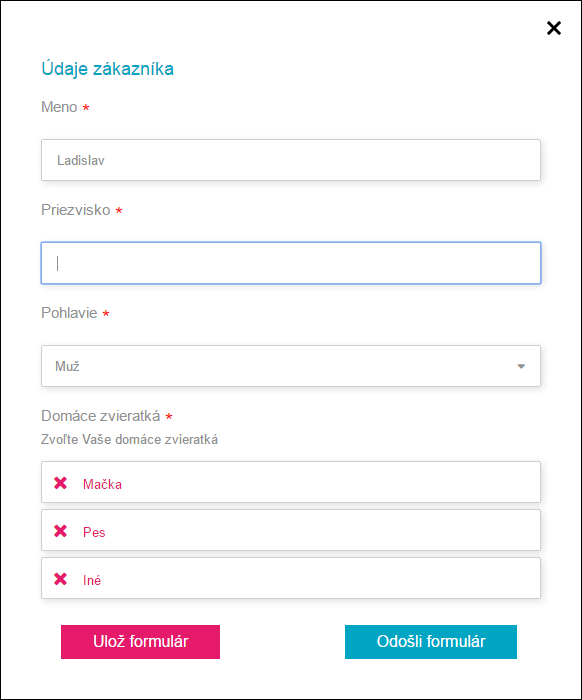
\includegraphics[width=0.7\linewidth]{images/kubko}
	\caption{Server formulárov a dátového modelu- Jakub Kováčik}
	\label{fig:Server formulárov a dátového modelu- Jakub Kováčik}
\end{figure}



\subsection{Server manažmentu rolí a používateľov}

	


	

